\documentclass[]{beamer}
%\usepackage[utopia]{mathdesign}
%\usepackage[no-math]{fontspec}
%\setmainfont{Liberation Serif}

\usepackage{minted}
% \usepackage{redhat}
\usepackage{hyperref}
\usepackage{ccicons}
\usepackage{ulem}

\hypersetup{
  colorlinks=true,
  linkcolor=blue,
}

\usepackage{tikz}
\usetikzlibrary{arrows,shapes,snakes,automata,backgrounds,petri}

%gets rid of bottom navigation bars
\setbeamertemplate{footline}[frame number]{}

%gets rid of navigation symbols
\setbeamertemplate{navigation symbols}{}

\usepackage[export]{adjustbox}

\newcommand{\done}{\textcolor{teal}{\checkmark}}
\newcommand{\pull}[3]{\href{https://github.com/systemd/#1/pulls/#2}{#3 (\##2)}}
\newcommand{\pulldone}[3]{\pull{#1}{#2}{#3} \done}
\newcommand{\commit}[3]{\href{https://github.com/systemd/#1/commit/#2}{#3 (#2)}}
\newcommand{\commitdone}[3]{\commit{#1}{#2}{#3} \done}
\newcommand\pp\pause
%\newcommand\pp{}

\newcommand{\flag}{
\includegraphics[height=1em]{images/flag.png}}

\title{\textsc{Rewriting \texttt{pyc} files for fun and reproducibility}}
\author{Zbigniew Jędrzejewski-Szmek}
\institute{%
  
\includegraphics[width=0.4\textwidth]{images/Logo-redhat-color-375.png}\\
  \medskip
  \textit{zbyszek@in.waw.pl}\\
  \medskip
  \ccbysa
}
\date{\tiny FOSDEM, Bruxelles/Brussel 2.2.2025}

\begin{document}

\setbeamertemplate{itemize items}[square]

\begin{frame}
  \titlepage % Print the title page as the first slide
\end{frame}

\begin{frame}
  \frametitle{About me}

  \begin{itemize}
  \item RedHatter working on systemd and various open source things
  \item Fedora contributor working on package build reproducibility
  \item Long time ago some small contributions to CPython
  \end{itemize}

  \vfill

  \hspace*{\fill}
  
\includegraphics[height=2em,width=2em]{images/Fedora_logo.png}
  
\includegraphics[height=2em,width=2em]{images/Fedora_logo.png}
  
\includegraphics[height=2em,width=2em]{images/Fedora_logo.png}
  
\includegraphics[height=2em,width=2em]{images/Fedora_logo.png}
  \hspace*{\fill}
\end{frame}

\begin{frame}
  \frametitle{What is build reproducibility?}

  \pause

  > \textit{A build is reproducible if given the same source code, build
  environment and build instructions, any party can recreate
  bit-by-bit identical copies of all specified artifacts.}
  
  \hfill – \href{https://reproducible-builds.org/docs/definition/}{reproducible-builds.org}

  \vfill
  \pause

  Two angles of motiviation:
  \begin{itemize}
  \item Security (independent verification of suply chain security)
  \item Quality (issues in hardware, build systems, packaging, software)
  \end{itemize}
\end{frame}

\begin{frame}
  \frametitle{How do we achieve build reproducibility?}

  \pause

  \begin{itemize}
  \item packages are built in a container with no network access
  \item dependencies are installed as packages
  \item build process must be determininistic
  \item operation independent of the environment (e.g. time clamped to \texttt{\$SOURCE\_DATE\_EPOCH})
  \end{itemize}

  \vfill
  \pause

  To solve issues that cannot be resolved by changing individual packages
  or tools, we apply a post-build cleanup…
\end{frame}

\begin{frame}[fragile]
  \frametitle{How do we achieve build reproducibility?}
  \framesubtitle{post-build cleanups}

  \pause

  Debian has \href{https://packages.debian.org/sid/dh-strip-nondeterminism}{\texttt{strip-nondeterminism}}\\
  Fedora now has \href{https://github.com/keszybz/add-determinism}{\texttt{add-determinism}}\\

  \vfill
  \pause

  \texttt{add-determinism} runs after the install phase of the package build

  {\tiny
  \begin{minted}{text}
+ /usr/bin/add-determinism --brp -j2 /builddir/build/BUILD/python-tables-3.10.1-build/BUILDROOT    
/…/BUILDROOT/…/tables/misc/__pycache__/__init__.cpython-313.pyc:
           rewriting with normalized contents
/…/BUILDROOT/…/tables/misc/__pycache__/enum.cpython-313.pyc:
           rewriting with normalized contents
...
Scanned 36 directories and 362 files,
               processed 94 inodes,
               94 modified (30 replaced + 64 rewritten),
               0 unsupported format, 0 errors
  \end{minted}
  }

  \vfill
  \pause

  \begin{itemize}
  \item \sout{ownership and mtimes in \texttt{*.zip}, \texttt{*.jar}, and \texttt{*.a} archives}
  \item \sout{timestamps in javadoc \texttt{*.html}}
  \item python \texttt{*.pyc} files
  \end{itemize}
\end{frame}

\begin{frame}
  \frametitle{}

  \hfill \large{The intro is finally over, phew!} \hfill{}
\end{frame}

\begin{frame}
  \frametitle{pyc files}
  \framesubtitle{i.e. the thing this talk is supposed to be about…}

  \pause
  \vfill

  \texttt{.py} source file → \texttt{.pyc} cached bytecode
  
  \pause
  \vfill

  \begin{itemize}
  \item CPython will (attempt to) write .pyc files every time\\
    it loads a .py file
  \item writing may fail
  \item Fedora packages include .pyc files for speed and reliability 
  \end{itemize}

  \vfill
\end{frame}

\begin{frame}
  \frametitle{pyc contents}
  \framesubtitle{basic objects}

  \pause

  [VERSION1 VERSION2 MAGIC1 MAGIC2 4–12 byte header]\\
  {}[object1] [object2] … [object…]

  \vfill
  \pause

  Object can be:\\\pause
  an 32-bit integer: ['i' BYTE4 BYTE3 BYTE2 BYTE1]\\\pause
  an 64-bit float: ['g' BYTE8 BYTE7 … BYTE2 BYTE1]\\\pause
  an 2×64-bit complex: ['y' REAL8 … REAL1 IMAG8 … IMAG1]\\\pause
  a Python integer: ['l' SIZE4 SIZE3 SIZE2 SIZE1\\
    \phantom{x} \hfill DIGIT1\_4 DIGIT1\_3 DIGIT1\_2 DIGIT1\_1\phantom{]}\\
    \phantom{x} \hfill … DIGITn\_1] \\\pause
  normal string: ['s'/'t'/'u'/'a'/'A' SIZE4 … SIZE1 CHAR1 ... CHARn]\hspace*{-1em}\\\pause
  short ASCII string: ['z'/'Z' SIZE CHAR1 … CHARn]\\\pause
  special Python stuff: ['N'/'F'/'T'/'.'/'S']
\end{frame}

\begin{frame}
  \frametitle{pyc contents}
  \framesubtitle{complex objects}

  \pause

  list: ['[' SIZE4 … SIZE1 [object1] … [objectn]]\\\pause
  tuple: ['(' SIZE4 … SIZE1 [object1] … [objectn]]\\\pause
  \phantom{tuple:} [')' SIZE [object1] … [objectn]]\\\pause
  sets: ['<'/'>' SIZE4 … SIZE1 [object1] … [objectn]]\\\pause
  dicts: ['\{' [key] [value] ...[key] [value] '0']\\\pause

  New in Python 3.14 — slice objects: [':' [start] [stop] [step]]
\end{frame}

\begin{frame}
  \frametitle{pyc contents}
  \framesubtitle{very complex objects}

  \pause

  code object: ['c' [ARGCOUNT] [POSONLYARGCOUNT] [KWONLYARGCOUNT] … [FLAGS] [code] [consts] [names] … [filename] [name] [qualname] …]
  \\\pause

  the whole pyc file:\\{}
  [VERSION1 VERSION2 MAGIC1 MAGIC2 4–12 byte header]\\
  \only<2>{[object1] [object2] … [object…]}%
  \only<3>{[code]}%
  \uncover<4->{[code [string1] [string2] ... [list ...]]}
\end{frame}



\begin{frame}
  \frametitle{pyc contents}
  \framesubtitle{reference objects}

  \pause

  reference: ['r' BYTE4 … BYTE1]

  \vfill
  \pause

  [HEADER] [object1] [object2 \flag] [object3] [object4 \flag] … \\{}
  ...\\\pause
  {}[REF 0] ... [object] ... [REF 1]
\end{frame}

\begin{frame}
  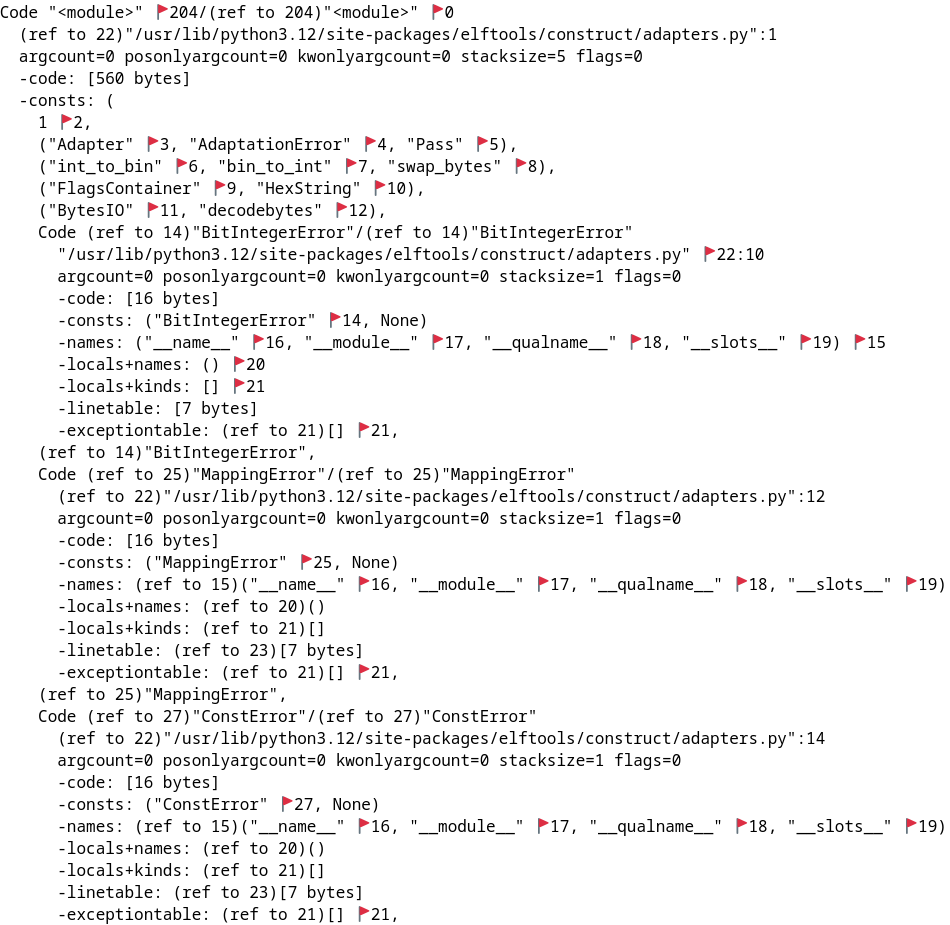
\includegraphics[width=\textwidth]{images/pyc-dump.png}
\end{frame}

\begin{frame}
  \frametitle{Irreproducibilities observed}

  \begin{itemize}
  \pause
  \item Only objects with \flag{} can be referenced

  \pause
  \item Objects may be flagged without being referenced\\
    → ``unused flags''

  \pause
  \item Not all objects have to replaced by references

  \pause
  \item Many different equivalent serializations
  \end{itemize}

  \vfill
  \pause

  Solution:\\\pause
  \begin{itemize}
  \item rewrite the object stream with minimal number of flags and maximal number of references
  \end{itemize}
\end{frame}

\begin{frame}
  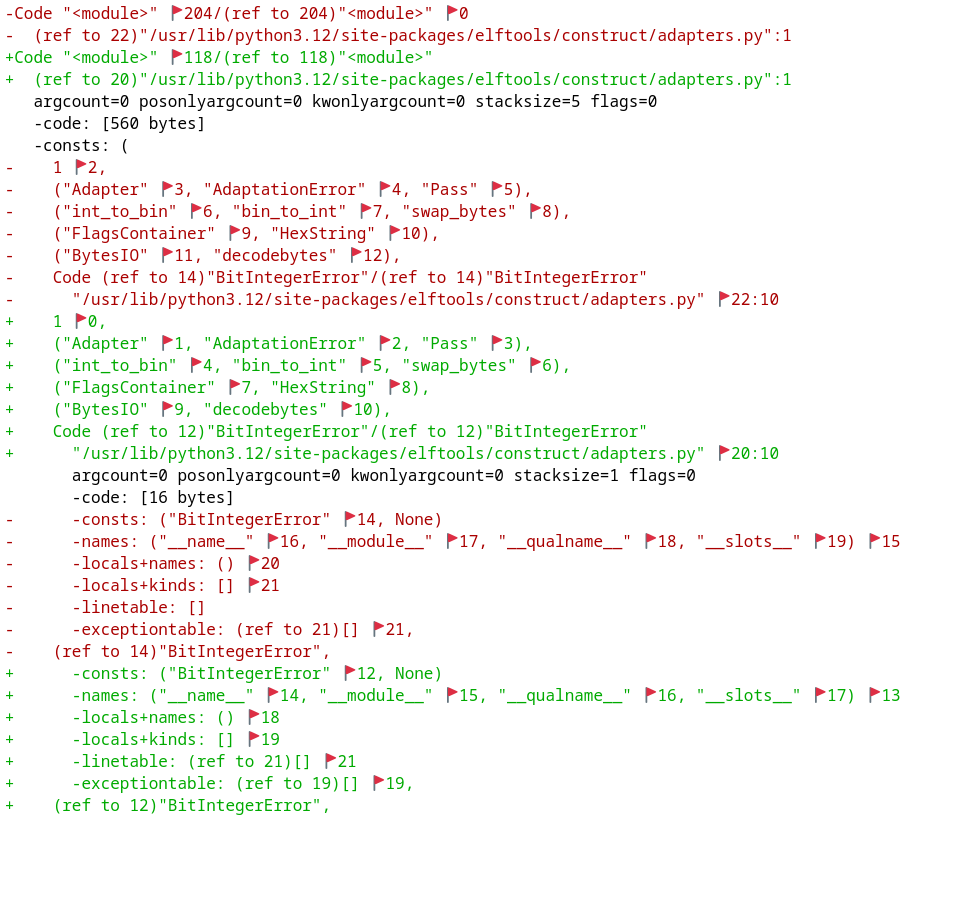
\includegraphics[width=\textwidth]{images/pyc-diff.png}
\end{frame}

\begin{frame}
  \frametitle{Questions \& further steps}

  \begin{itemize}
    \pause
  \item CPython could be improved to … maximize references and minimize flags
    \pause
  \item Is it OK to reference mutable objects?
    \pause
  \item Can we change 's' → 'z'? (3 bytes less, more references)
    \pause
  \item Can we change 'A'/'Z' → 'a/'z'? (more references)
    \pause
  \item Can we change 'l' → 'i'? (4 bytes less, simpler processing, more references)
    \pause
  \item Can we change '[' ←→ '('/')'? (more references, less bytes)
  \end{itemize}

  \begin{itemize}
    \pause
  \item \texttt{add-determinism -p} is useful\pause, but no bytecode decoder
    \pause
  \item \texttt{diffoscope} should use \texttt{marshalparser -p}/\\
      \texttt{marshal-parser -p}/\texttt{add-determinism -p}
  \end{itemize}
\end{frame}

\begin{frame}
  \frametitle{Links and references}
  
  For more info:
  \begin{itemize}
  \item \href{https://reproducible-builds.org}{reproducible-builds.org}
  \item \href{https://fedoraproject.org/wiki/Changes/ReproduciblePackageBuilds}{Fedora ReproduciblePackageBuilds Change}
  \item \href{https://www.youtube.com/watch?v=nJHh-VJnGt8}{Flock 2024 Reproducible builds in Fedora} talk
  \end{itemize}

  Tools:
  \begin{itemize}
  \item \href{https://github.com/keszybz/add-determinism}{github.com/keszybz/add-determinism}
  \item \href{https://packages.debian.org/sid/dh-strip-nondeterminism}{packages.debian.org/sid/dh-strip-nondeterminism}
  \item \href{https://github.com/fedora-python/marshalparser}{github.com/fedora-python/marshalparser}
  \item \href{https://crates.io/crates/marshal-parser}{crates.io/crates/marshal-parser}
  \end{itemize}
\end{frame}

\end{document}
